\documentclass[a4paper,10pt]{report}
\usepackage[utf8x]{inputenc}
\usepackage[francais]{babel}
\usepackage{fullpage}
\usepackage[none]{hyphenat}
\usepackage{listings}
\usepackage{url}
\usepackage{graphics}

% Title Page
\title{Communication}
\author{Maxime COLIN}


\begin{document}
\maketitle

\begin{abstract}
Ce document présente les différentes technologies envisagées pour notre projet.
\end{abstract}


\chapter{Compatibilité}


\chapter{Client}




\section{HTML5}
HTML5 est la dernière version de HTML, il introduit dans ses spécifications plusieurs 
balises, 
de nouveaux types et attributs pour les anciennes balises. 
On pourrait implémenter la majorité des fonctionnalités qu'on souhaite en HTML, couplé 
avec CSS et JavaScript, mais ce langage n'est pas fait pour nos besoins, et on va donc 
chercher d'autres solutions plus adaptées. 

\section{Canvas}
Canvas est un composant de HTML5 qui permet d'effectuer des rendus dynamiques d'images 
bitmap via des scripts.
Canvas se résume donc en une zone de dessin dont la hauteur et la largeur sont définies 
dans du code HTML. Du code javascript permet d'accéder à l'aire via une série complète de fonctions de dessins, 
similaires aux autres API 2D, bien que permettant de générer dynamiquement des graphismes. Certaines personnes ont anticipé cet emploi de canvas en l'utilisant pour des graphiques, des animations et de la création d'images.
Le composant canvas est plutôt récent et n'est pour le moment implémentée que par 
quelques navigateurs: Firefox, Opéra, Safari, Konqueror, Google Chrome. 
Internet Explorer est encore en retard là-dessus mais l'arrivée de IE 9 permettra
 de le rattraper.

\begin{itemize}
  \item{Points forts}
Dans un contexte hautement dynamique, la légèreté des images bitmap permet un traitement
 plus rapide des graphiques.
\item{Points faibles}
 \begin{itemize}
\item La qualité des graphiques baisse en fonction de la taille de l'écran.
\item Très jeune âge.
\end{itemize}
\end{itemize}


 Sources:
\begin{itemize}
\item \url{http://fr.wikipedia.org/wiki/Canvas_(HTML)}
\item \url{https://developer.mozilla.org/fr/HTML/Canvas}
\end{itemize} 
	  

\section{SVG}
SVG est un format de données conçu pour décrire des ensembles de graphiques vectoriels. 
Il est basé sur XML. Les coordonnées, dimensions et structures de ces graphiques 
vectoriels sont indiqués sous forme numérique dans le document XML. 
Les couleurs et les polices de caractères à utiliser sont gérées par 
les feuilles de styles. 
En plus de la gestion de formes basiques (rectangles, ellipses, etc.), SVG gère
 des chemins (paths), qui utilisent les courbes de Bézier et qui permettent ainsi
 d'obtenir presque n'importe quelle forme.  D'autres outils lui permettent de gérer 
également le remplissage et la transparence des graphiques.

\begin{itemize}
\item Points forts
\begin{itemize}
\item Les graphiques vectoriels permettent de s'adapter aux différentes tailles d'écran, 
i.e. graphiques de très bonne qualité en toute circonstance.
\item Disponibilité de bibliothèques Javascript qui proposent des fonctionnalités de base 
et permettent de faciliter le travail des développeurs (i.e. raphael.js).
\item Il existe des logiciels graphiques qui permettent de modifier facilement chaque
 forme, par exemple en déplaçant des points, ou en changeant la couleur des traits, etc.
\end{itemize}
\item Points Faibles
\begin{itemize}
\item Le revers de la médaille de la qualité du graphisme est évidemment la consommation 
accrue de CPU (proportionnelle à la taille du graphique),
\item Rendement très faible dans un contexte très dynamique.
\item Ne permet pas de créer des points d'articulations, tels des nœuds dans un graphe. 
Bref, la notion de pointeur n'existe pas en SVG, ce qui rend la description de scènes 
dynamiques complexe.
\end{itemize} 
\end{itemize} 

Sources:\url{http://fr.wikipedia.org/wiki/Scalable_Vector_Graphics}

\section{Flash}
Les fichiers Flash, généralement appelés « animation Flash » portent l'extension .swf. 
Ils peuvent être inclus dans une page web et lus par le plugin Flash du navigateur, ou 
bien interprétés indépendamment dans le lecteur Flash Player. Flash est incontestablement 
une des méthodes les plus populaires pour ajouter des animations et des objets
 interactifs à une page web. 
Cependant, si Flash est une technologie très adaptée à nos besoins, elle est propriétaire
 et n'est donc pas compatible avec notre volonté de faire du « Web Ouvert ».
 
Sources : 
\begin{itemize}
\item  \url{http://pro.clubic.com/creation-de-site-web/langage-programmation/actualite-334796-cs5-flash-canvas-html5.html}
\item \url{http://fr.wikipedia.org/wiki/Adobe_Flash#Flash_et_le_.C2.AB_Web_.C2.BB}
\end{itemize}

\section{Comparatif}
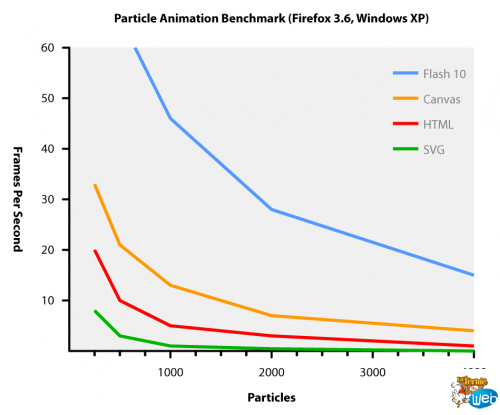
\includegraphics{bench.png}
Le graphique ci-dessous nous donne un comparatif des quatre technologies dans 
un contexte très dynamique.
 
Le graphique ci-dessus donne un comparatif du rendement de ces quatre technologies sous 
Firefox (résultat similaire pour les autres navigateurs) et le résultat est sans appel: 
Flash l'emporte haut la main, canvas vient en deuxième position, HTML et SVG en dernière 
position.

  

Le lien suivant donne un comparatif en image du rendement de ces technologies:
 
\url{http://www.lafermeduweb.net/billet/un-bench-flash-vs-canvas-comparant-une-animation-de-particules-801.html}

\section{Conclusion}
Malgré la puissance de Flash, nous avons décidé de ne pas utiliser cette 
technologie pour rester dans l'esprit de l'open source.
Dans le contexte de notre moteur de jeux qui n'est pas très dynamique, le large panel 
d'outils offert par SVG, grâce à son ancienneté et la qualité de ses graphiques,
 nous incite à choisir cette technologie. De plus, elle est largement supportée par les navigateurs
 (cf. Etude sur la compatibilité). 
















\chapter{Serveur}


\chapter{Communication}

Cette partie concerne les technologies de communication client/serveur et 
client/client. Les différentes pistes retenu sont les WebSockets, Ahax, 
Opera Unite.

  \section{WebSocket}

    \subsection{Présentation}

WebSocket est une technologie fournissant un canal de communication bidirectionnel 
et fullduplex à travers un socket TCP. Il a été conçu pour être implémenté dans 
les navigateurs et serveurs web, mais il peut être utilisé n'importe quelle 
application client ou serveur. L'API WebSocket est en phase de standardisation 
par le W3C et le protocole par IETF.


Un tel canal de communication permet :
\begin{itemize}
  \item la notification au client d'une modification d'état du serveur
  \item l'envoie de données du serveur au client sans que celui ci n'ai à faire de requête
\end{itemize}


    \subsection{Implémentation et support coté client}

Le protocoles WebSocket est implémenté dans les navigateurs Chrome 4, Safari 5, 
Firefox 4 et Opera 11. Son support est néanmoins désactivé dans Firefox 4 et 
Opera 11 pour de raison de sécurité. Il est possible de l'activé via dans les 
paramètres des deux navigateurs. Internet Explorer ne supporte pas WebSocket.


    \subsection{Implémentation et support coté serveur}

Le protocole nécessite également d'être implémenté côté serveur pour être 
utilisé. Il existe plusieurs implémentations côté serveur de WebSocket, 
dans différents langages (Java, Python, PHP, Javascript, ...) et sous 
différentes formes (extension apache, serveur entier, script, ...).


Quelques implémentations :
\begin{itemize}
  \item GNU WebSocket4J, une implémentation du protocole WebSocket en Java. 
  \item pywebsocket3, une implémentation en Python sous la forme d'une extension pour le serveur  Apache.
  \item jWebSocket, implémentation Java côté serveur et JavaScript/HTML5 côté client.
  \item Implémentation de WebSocket avec node.js
\end{itemize}


    \subsection{Sécurité}

WebSocket comporte à l'heure actuel une faille de sécurité dans la phase 
de ``handshacke'' permettant de remplacer un fichier javascript par un malware. 
La faille se situe au niveau de l'API elle même. C'est pourquoi son support 
est désactivé par défaut Firefox 4 et Opera 11 jusqu'à ce que la faille 
soit comblé.


  \section{Ajax}

    \subsection{Présentation}

Ajax (Asynchronous Javascript and XML) est un rassemblement de different outils 
et méthode de conception permettent de construire des application web dynamique 
basé sur différentes technologies web côté client.

Ajax est une combinaison de technologie telle que JavaScript, CSS, XML, DOM et 
XMLHttpRequest dans le but de réaliser des applications Web qui offrent une 
maniabilité et un confort d'utilisation supérieur à ce qui se faisait jusqu'alors.

DOM et JavaScript sont utilisés pour modifier l'information présentée dans le navigateur 
par programmation. L'objet XMLHttpRequest est utilisé pour dialoguer de manière 
asynchrone avec le serveur Web. La notation XML est utilisée pour structurer les 
informations transmises entre le serveur Web et le navigateur.

En alternative au format XML, les applications Ajax peuvent utiliser les fichiers texte ou JSON.

  \subsection{Support}

Les applications Ajax fonctionnent sur tous les navigateurs Web qui mettent en oeuvre les 
technologies décrites précédemment, parmi lesquels Mozilla Firefox, Internet Explorer, 
Konqueror, Google Chrome, Safari et Opera.


  \section{Opera Unite}

    \subsection{Présentation}

Opera Unite est une technologie qui transforme un navigateur en serveur 
Web personnel. Avec Opera Unite, on devient à la fois client et serveur, 
à la fois visiteur et hôte. On reçoit du contenu du Web, et on en fournit 
également. On garde le contrôle : les données restent sur votre ordinateur, 
et on décide avec qui on désire les partager. 

    \subsection{Implémentations}

Opera Unite est implémenté dans le navigateur Opera depuis la version 10.


    \subsection{Conclusion sur Opera Unite}

Opera Unite est au final un service de partage de contenu et non de 
communication client/serveur, cette solution est donc inadaptée à nos 
besoins. De plus, cette fonctionnalité n'est disponible que sur le 
navigateur Opera.

  \section{Conclusion}

En conclusion, la technologie WebSocket semble la plus intéressante pour notre projet.
Elle semble adapté à nos besoins. Néanmoins le fait que le protocoles soit 
encore en phase de développement et le fait qu'il soit désactivé par défaut 
sur certains navigateurs pourrait poser problème.

Ajax semble également correspondre à certaines de nos attentes, mais dispose de plus
de restriction au niveau communication client/serveur.

\chapter{Formats de données}

  \section{JSON}

    \subsection{Présentation}

JSON (JavaScript Object Notation) est un format de données textuel, 
générique, dérivé de la notation des objets du langage ECMAScript. 
Il permet de représenter de l’information structurée. Créé par Douglas 
Crockford, il est décrit par la RFC 4627 de l’IETF.


Un document JSON ne comprend que deux éléments structurels : 
\begin{itemize}
 \item des ensembles de paires nom / valeur ; 
 \item des listes ordonnées de valeurs. 
\end{itemize}


Ces mêmes éléments représentent 3 types de données : 
\begin{itemize}
  \item des objets ; 
  \item des tableaux ; 
  \item des valeurs génériques de type tableau, objet, booléen, nombre, chaîne ou null. 
\end{itemize}

Le format JSON est très facilement exploitable et manipulable en Javascript. 
Un document JSON représente un objet. Il est donc potentiellement plus facile 
à manipuler qu'un document XML.

    \subsection{Exemple}

\begin{verbatim}
{"menu": {
   "id": "file",
   "value": "File",
   "popup": {
     "menuitem": [
       {"value": "New", "onclick": "CreateNewDoc()"},
       {"value": "Open", "onclick": "OpenDoc()"},
       {"value": "Close", "onclick": "CloseDoc()"}
     ]
   }
 }}
\end{verbatim}

    \subsection{Sources}

\begin{itemize}
 \item \url{http://fr.wikipedia.org/wiki/Json}
\end{itemize}


  \section{XML}

    \subsection{Présentation}

Extensible Markup Language est un langage informatique de balisage générique. 
Il sert essentiellement à stocker/transférer des données de type texte Unicode 
structurées en champs arborescents. Ce langage est qualifié d’extensible car 
il permet à l'utilisateur de définir les balises des éléments. L'utilisateur 
peut multiplier les espaces de nommage des balises et emprunter les définitions 
d'autres utilisateurs

    \subsection{Exemple}

\begin{verbatim}
<menu id="file" value="File">
  <popup>
    <menuitem value="New" onclick="CreateNewDoc()" />
    <menuitem value="Open" onclick="OpenDoc()" />
    <menuitem value="Close" onclick="CloseDoc()" />
  </popup>
</menu>
\end{verbatim} 

    \subsection{Sources}

\begin{itemize}
 \item \url{http://fr.wikipedia.org/wiki/Xml}
\end{itemize}


  \section{HTML}

    \subsection{Présentation}

L’Hypertext Markup Language, généralement abrégé HTML, est le format de données 
conçu pour représenter les pages web. C’est un langage de balisage qui permet 
d’écrire de l’hypertexte, d’où son nom. HTML permet également de structurer 
sémantiquement et de mettre en forme le contenu des pages, d’inclure des 
ressources multimédias dont des images, des formulaires de saisie, et des 
éléments programmables tels que des applets. Il permet de créer des documents 
interopérables avec des équipements très variés de manière conforme aux exigences 
de l’accessibilité du web.

    \subsection{Sources}

\begin{itemize}
 \item \url{http://fr.wikipedia.org/wiki/Json}
\end{itemize}

  \section{Conclusion}

JSON et XML sont les deux format qui semble les plus adaptés à nos besoin. 
JSON à un avantage au niveau de son interprétation par Javascript, une 
technologie certainement clé dans ce projet.

\chapter{Webographie}

  \section{Delicious}

Mon compte delicious : \url{http://www.delicious.com/binome.lyon/wge}


\end{document}          
